%%%%%%%%%%%%%%%%%%%%%%%%%%%%%%%%%%%%%%%%%%%%%%%%%%%%%%%%%%%%%%%%%%%%%%%%%%%
%
%  para un artículo en LaTeX en español.
%
%%%%%%%%%%%%%%%%%%%%%%%%%%%%%%%%%%%%%%%%%%%%%%%%%%%%%%%%%%%%%%%%%%%%%%%%%%%
\documentclass[]{article}
% Esto es para poder escribir acentos directamente:
\usepackage[latin1]{inputenc}
% Esto es para que el LaTeX sepa que el texto está en español:
\usepackage[spanish]{babel}
%para cambiar los margenes del texto
\usepackage[a4paper,left=3cm,right=2cm,top=2.5cm,bottom=2.5cm]{geometry}
\usepackage{hyperref}
\usepackage{graphicx}
\graphicspath{ {images/} }
% Paquetes de la AMS:
%\usepackage{amsmath, amsthm, amsfonts,float}
\graphicspath{ {../Tarea_1/} }


%--------------------------------------------------------------------------
\title{Reporte pr�ctica uno: Movimiento Browniano}
\author{Jos� Anastacio Hern�ndez Salda�a\\
  \small Posgrado de Ingenier�a de Sistemas\\
  \small 1186622\\ 
  \small jose.hernandezsld@uanl.edu.mx
}

\begin{document}

\maketitle

\abstract{Este es un reporte sobre la pr�ctica uno de movimiento browninano que se realiz� en la clase de Simulaci�n de Sistemas, c�mputo paralelo en R.}

\section{Introducci�n}

El Movimiento Browniano se refiere a una part�cula que cambia su posici�n uniformemente al azar. Los movimientos pueden ser de diferentes tipos, pero en esta pr�ctica nos limitamos a el caso sencillo donde una part�cula se mueve en pasos discretos, es decir, cada paso mide lo mismo, y las �nicas posibles direcciones de movimiento son las direcciones paralelas a los ejes cardinales del sistema de coordenadas en el cual se realiza el movimiento. Vamos a utilizar pasos unitarios (es decir, cada paso mide uno), teniendo como la posici�n inicial el origen. 
\\\\
Lo que se busc� obtener es analizar de una manera sistem�tica los efectos de la dimensi�n en el n�mero de veces que la caminata pasa por el origen, verificando que el tama�o de la caminata y el n�mero de repeticiones del experimento no causen un efecto significativo en el an�lisis.
\section{Dise�o del Experimento}
Tomando como base el c�digo de ejemplo en la \href{http://elisa.dyndns-web.com/teaching/comp/par/p1.html}{p�gina del curso} donde se realiza una caminata aleatoria y calcular su distancia, se modific� para que registrara el n�mero de veces que pasa por el origen durante la caminata, implement�ndose un paralelizaci�n de la experimentaci�n. se har�n variar los valores de n�mero de repeticiones y la duraci�n de la caminata para poder tener los datos necesarios y poder realizar el an�lisis estad�stico.
\\\\
Se comenz� con un primer vistazo al comportamiento de la caminata variando las dimensiones de uno a ocho con 200 repeticiones y caminatas de 300 pasos de duracion obteniendo el resultado de la figura \ref{fig::figura1}
\\\\
\begin{figure}
  \centering
  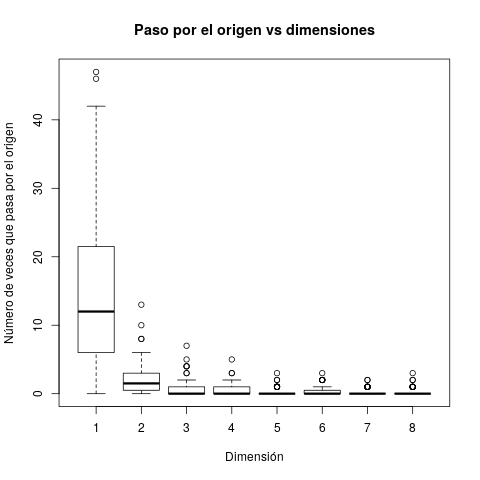
\includegraphics[width=0.26\textheight]{PasoPorOrigen}
  \caption{200 repeticiones y duraci�n de 300}
  \label{fig::figura1} 
\end{figure}

Para el experimento se variaron las dimensiones de una a ocho, repiti�ndose el experimento 50, 100, 150 y 200 veces con duraciones de caminata de 100, 150, 200, 250 y 300 pasos. 

Teniendo una vez la informaci�n necesaria, se realizo una prueba de normalidad a partir de una regresi�n lineal simple a los datos y revisando sus residuos, como se contaban con mas de 5,000 datos dentro de la poblaci�n fue necesario hacer una muestra de 5000 y compararla con la distribucion de la poblacion, quedando el histograma de los residuos de las siguientes figuras \ref{fig::figura2}  \ref{fig::figura3}.
\\\\
\begin{figure}
  \centering
  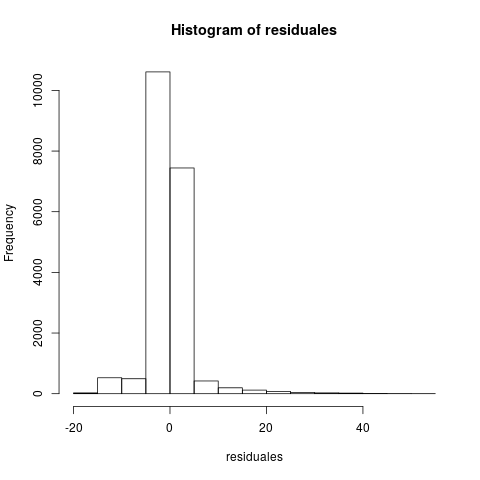
\includegraphics[width=0.26\textheight]{residuales}
  \caption{histograma de los residuales de la poblacion}
  \label{fig::figura2} 
\end{figure}

\begin{figure}
  \centering
  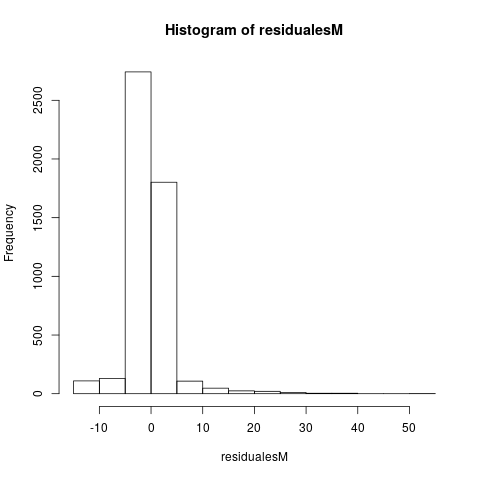
\includegraphics[width=0.26\textheight]{residualesMuestra}
  \caption{histograma de los residuales de la muestra}
  \label{fig::figura3} 
\end{figure}

Los residuales aparentan no tener una distribucion normal, por lo que se hizo una prueba de Shapiro-Wilk a la muestra para corroborarlo.

	Shapiro-Wilk normality test
\\\\
data:  residualesMuestra
\\
W = 0.6048, p-value $<$ 2.2e-16
\\
Como la prueba arrojo un valor de p muy cercano a cero, se rechaza la hipotesis nula de que la muestra de los residuales venga de una distribucion normal. por lo que no se podria realizar una an�lisis de varianza, sino tendria que recurrirse a pruebas no parametricas.
\\\\
Se aplico a la poblacion de los datos la prueba Kruskal-Wallis para poder saber si hay una relacion entre el numero de cruces y las repeticiones del experimento y la duracion de la caminata.

	Kruskal-Wallis rank sum test
\\\\
data:  datos\$crxs by datos\$iteration
\\
Kruskal-Wallis chi-squared = 3.5127, df = 3, p-value = 0.3191
\\\\

	Kruskal-Wallis rank sum test
\\\\
data:  datos\$crxs by datos\$duration
\\
Kruskal-Wallis chi-squared = 5.6359, df = 4, p-value = 0.228
\\\\

Al revisar el valor de p por encima de un valor significativo de alfa, la hipotesis nula de que las medias de los factores de las iteracion y la duracion son iguales, por lo que no afectan el numero de cruces.

\section{Conclusiones}

Como se pud� observar desde el principio, el numero de cruces por el origen de una caminata aleatoria de movimiento browneano no se ve afectado por el largo de la caminata o el numero de repeticiones del experimento, y si se ve afectado por el numero de dimensiones en donde hace el movimiento.

\end{document}
